\documentclass[a4paper,fontset = windowsnew]{ctexbook}
\usepackage{xifthen}
\usepackage{calc}
\usepackage{graphicx}
\usepackage{tikz}
\usepackage{cexam}

\begin{document}
\chapter{基本排版程序}

\ExplSyntaxOn

\parindent=0pt

% 选择题数据结构探测det 指 detect
%%%%
\bool_new:N \sel_data_bool
\cs_new:Npn \sel_data_det:n #1
{
% 默认无选择题结构
  \bool_set_false:N \sel_data_bool
% 对四个选项的探测
  \str_if_in:nnTF {#1}{A.}
  {
    \str_if_in:nnTF {#1}{B.}
    {
      \str_if_in:nnTF {#1}{C.}
      {
	\str_if_in:nnTF {#1}{D.}
	{\bool_set_true:N \sel_data_bool}
	{\relax}
      }
      {\relax}
    }
    {\relax}
  }
  {
    {\relax}
  }
}
% 图片探测
\cs_new:Npn \cexam_pic_det:n #1
{
% 默认无图片
  \bool_set_true:N \cexam_nopic_bool
% 对图片的探测
  \str_if_in:nnTF {#1}{<:}
  {
    \str_if_in:nnTF {#1}{:>}
    {\bool_set_false:N \cexam_nopic_bool}
    {\relax}
  }
  {\relax}
}
%% 此命令用以取代\cexam_sep_pictxt_ii:n
\cs_new:Npn \cexam_sep_pictxt_iii:n #1 
{
  \cexam_pic_det:n {#1}
  \bool_if:NTF \cexam_nopic_bool
  {
    \cs_set:Nn \cexam_seped_pic: {}
    \cs_set:Nn \cexam_seped_txt: {#1}
  }
  {
    \cexam_sep_pictxt:n \relax #1\relax\scan_stop:
  }
}
%排版依据
\dim_new:N \sel_optpic_hti_dim
\box_new:N \sel_optpic_box
\dim_new:N \sel_optpic_wd_dim
\dim_new:N \sel_optpic_ht_dim
% 题号
\int_new:N \cexam_number_int
\box_new:N \cexam_number_box
% 首行缩进
\dim_new:N \cexam_indent_dim
\dim_new:N \cexam_indent_i_dim
%%%%%%%%%%%%%%%%%%%%%%%%%%%%%%%%%%%%%%%%%%%%%%%%%%%%%%%%%%%%%%%%%%%%%%%%
%%%%%%%%%%%%%%%%%%%%%%%%%%%%%%%%%%%%%%%%%%%%%%%%%%%%%%%%%%%%%%%%%%%%%%%%
% 选择题排版
\cs_new:Npn \selection_type:n #1.#2 A.#3 B.#4 C.#5 D.#6 \scan_stop:
{
% 设置题号决定的缩进
  \int_add:Nn \cexam_number_int {1}
  \hbox_set:Nn \cexam_number_box {\int_use:N \cexam_number_int .}
  \dim_set:Nn \cexam_indent_dim{\box_wd:N \cexam_number_box}
  \dim_add:Nn \cexam_indent_dim{5pt}
  \dim_set:Nn \cexam_indent_i_dim {\cexam_indent_dim}
  \dim_add:Nn \cexam_indent_i_dim {1.23\ccwd}
% 分离图片和文字
  \cexam_sep_pictxt_iii:n {\cexam_ind_hat:nn {\cexam_indent_dim}{\int_use:N \cexam_number_int}#2} 
%  获得图片宽高
  \bool_if:NTF \cexam_nopic_bool
  {\relax}
  {
    \hbox_set:Nn \sel_optpic_box{\cexam_seped_pic:}
    \dim_set:Nn {\sel_optpic_wd_dim}{\box_wd:N \sel_optpic_box}
    \dim_set:Nn {\sel_optpic_ht_dim}{\box_ht:N \sel_optpic_box}
    \dim_add:Nn {\sel_optpic_ht_dim}{\box_dp:N \sel_optpic_box}
% 加入*号图片不加标号
    \str_if_in:nnTF {#1}{*}
    {\bool_set_false:N \cexam_fmt_bool}
    { 
      \bool_set_true:N \cexam_fmt_bool
      \dim_add:Nn \sel_optpic_ht_dim {\baselineskip}
    }
  }
%-->ok
% 据图片给出排版依据的高度
  \dim_set:Nn \sel_optwd_dim {\linewidth}
  \dim_sub:Nn \sel_optwd_dim {\cexam_indent_dim}
  \bool_if:NTF \cexam_nopic_bool
  {
    \cexam_fmt_opt_sel:nnnn {#3}{#4}{#5}{#6}
  }
  { 
    \dim_sub:Nn \sel_optwd_dim {\sel_optpic_wd_dim}
    \cexam_fmt_opt_sel:nnnn {#3}{#4}{#5}{#6}
% 取得文本高度
    \cexam_get_txtht:nno 
    {\sel_optpic_hti_dim}
    {\sel_optwd_dim}
    {\cexam_seped_txt:}
  }
% 准备排版
  \bool_if:NTF \cexam_nopic_bool
% 排版无图模式
  { 
    \bool_if:NTF \sel_opt_maxed_bool
    {
      \cexam_type_v:nnnnn 
      {\cexam_indent_dim}{0pt}
      {\cexam_indent_i_dim}{0pt}
      {\cexam_seped_txt:}
    }
    {
      \cexam_type_v:nnnnn 
      {\cexam_indent_dim}{0pt}
      {\cexam_indent_dim}{0pt}
      {\cexam_seped_txt:}
    }
    \newline
    \hbox_unpack:N \cexam_option_box
  }
% -->ok
% 排版含图模式
  {
    \dim_compare:nNnTF {\sel_optpic_hti_dim} > {\sel_optpic_ht_dim}
    {
% 给选项宽付值
      \dim_add:Nn \sel_optwd_dim {\sel_optpic_wd_dim}
      \cexam_fmt_opt_sel:nnnn {#3}{#4}{#5}{#6}
% 开始排版
% 四个选项缩进排版,三级缩进为2\ccwd
% 四个选项无缩进排版,三级缩进为\ccwd
      \bool_if:NTF \sel_opt_maxed_bool
      {\relax}
      {\dim_set:Nn \cexam_indent_i_dim {\cexam_indent_dim}}
      \cexam_type_ii:nnnnnnnnn
      {r}{\cexam_seped_pic:}
      {\cexam_indent_dim}{5pt}
      {\cexam_indent_dim}{0pt}
      {\cexam_indent_i_dim}{0pt}
      {\cexam_seped_txt:}
      \newline
      \hbox_unpack:N \cexam_option_box
    }
    {
% 判断排版格式
      \dim_sub:Nn \sel_optpic_ht_dim {\sel_optpic_hti_dim}
      \bool_if:NTF \sel_opt_maxed_bool
      { 
% 加入定义,以防止进入测定行数程序时的第一次展开
	\cs_set:Nn \cexam_seped_txt_i: 
	{\hbox_unpack:N \cexam_option_box}
%% 这个情况是选项过长问题,所以不必重新生成选项结构,直接一步改变选项宽度即可
	\dim_add:Nn \sel_optwd_dim {\sel_optpic_wd_dim}
	\cexam_type_iv:nnnnnnnn
	{r}{\cexam_seped_pic:}
	{\cexam_indent_dim}{5pt}
	{\cexam_indent_i_dim}{0pt}
	{\cexam_seped_txt:}{\cexam_seped_txt_i:}
      }
      {
	\dim_compare:nNnTF {\sel_optpic_ht_dim} > {2\baselineskip}
	{
	  \dim_add:Nn \sel_optwd_dim {\sel_optpic_wd_dim}
	  \cexam_fmt_opt_sel:nnnn {#3}{#4}{#5}{#6}
% 进入图片居于题干和选项之间居中排版
	  \cexam_type_iii:nnnnnnn
	  {c}{\cexam_seped_pic:}
	  {\cexam_indent_dim}{0pt}
	  {\cexam_indent_dim}{0pt}
	  {\cexam_seped_txt:}
	  \newline
	  \hbox_unpack:N \cexam_option_box
	}
	{
% 进入选项无缩进排列
	  \cexam_type_i:nnnnnnn
	  {r}{\cexam_seped_pic:}
	  {\cexam_indent_dim}{5pt}
	  {\cexam_indent_dim}{5pt}
	  {
	    \cexam_seped_txt:
	  }
	  \newline
	  \hbox_unpack:N \cexam_option_box
	}
      }
    }
  }
}
%%%%%%%%%%%%%%%%%%%%%%%%%%%%%%%%%%%%%%%%%%%%%%%%%%%%%%%%%%%%%%%%
%%%%模块测试
这是参考文本
这是参考文本
这是参考文本
这是参考文本
这是参考文本
这是参考文本
这是参考文本
这是参考文本
这是参考文本
这是参考文本
这是参考文本
这是参考文本
这是参考文本
%\int_set:Nn \cexam_number_int {100}
\par
\selection_type:n 
1.这是选择题的题干
这是选择题的题干
这是选择题的题干
\begin{equation}
%$$
%\[
  E=MC^2
%\]
%$$
\end{equation}
这是选择题的题干
这是选择题的题干
这是选择题的题干
这是选择题的题干
如~
<:
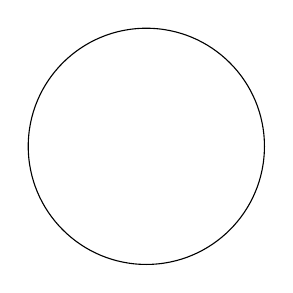
\begin{tikzpicture}
  \draw circle [radius=1.5];
\end{tikzpicture}
:>
所示是插入的图片,请选出正确的答案
所示是插入的图片,请选出正确的答案
A.这是选项A选项A选项A选项A选项A选项A选项A选项A选项A选项A选项A选项A选项A选项A选项A选项A选项A选项A选项A选项A选项A选项A选项AA选项A选项AA选项A选项AA选项A选项AA选项A选项AA选项A选项AA选项A选项A
B.这是选项B
C.这是选项C
D.这是选项D
\scan_stop:


\end{document}
